\section{Auswertung}
\label{sec:Auswertung}
\subsection{Berechnung der Grenzfrequenzen aus der Durchlasskurve}
Zunächst wird, wie in der Durchführung beschrieben, die Spannungsamplitude am Ende der $LC$-Kette in Abhängigkeit der Frequenz betrachtet.
Der mithilfe des $XY$-Schreibers entstandene Graph ist in Abbildung \ref{fig:durchlass} dargestellt.
Auf der $y$-Achse ist die Spannungsamplitude, auf der $x$-Achse der natürliche Logarithmus der Frequenz dargestellt.
Exemplarisch wurden an der $x$-Achse mehrere Frequenzwerte eingetragen, wobei diese den realen Frequenzwert und nicht dessen Logarithmus darstellen.
Um nun die Grenzfrequenzen möglichst genau ablesen zu können, wird eine lineare Regression durchgeführt.
Diese wird für die Längeneinheiten auf der $x$-Achse und die Logarithmen der Frequenzen für die abgelesenen Werte durchgeführt.
Alle abgelesenen Werte sind wiederum nochmals in Tabelle \ref{tab:durchlass} angegeben.\\
\begin{figure}
  \centering
  \includegraphics[angle=90, width=\textwidth]{aderlasskurve.png}
  \caption{Aufgenommene Durchlasskurve der alternierenden Kette.}
  \label{fig:durchlass}
\end{figure}
\begin{table}
  \centering
  \caption{Exemplarisch abgelesene Frequenzen der Durchlasskurve der $LC$-Kette.}
  \label{tab:durchlass}
  \sisetup{table-format=1.2}
  \begin{tabular}{c c}
    \toprule
    {$LE [\si{\centi\metre}]$} & {$\nu [\si{\kilo\hertz}]$}\\
    \midrule
    \input{build/atabelle.tex}
    \bottomrule
  \end{tabular}
\end{table}
Die lineare Regression wird nun mit der Methode der kleinsten Quadrate mit Hilfe von SciPy durchgeführt.
Es ergeben sich die Parameter
\begin{align*}
  b &= \input{regres_b.tex}, \\
  m &= \input{regres_m.tex}.
\end{align*}
Die Grenzfrequenzen werden an der Durchlasskurve zu
\begin{align*}
  g_1 &= \SI{9}{\centi\metre} \\
  g_2 &= \SI{16.5}{\centi\metre}
\end{align*}
abgelesen.
Aus diesen Längenangaben und den in der linearen Regression bestimmten Parametern ergibt die Umrechnungsformel
\begin{equation}
  \nu = \mathrm{e}^{m g_i + b}
\end{equation}
die gesuchten Grenzfrequenzen.
Vergleicht man diese mit den aus Formel \ref{eqn:grenzfrequenzen} bestimmten theoretischen Grenzfrequenzen, ergeben sich die Werte
\begin{align*}
  \nu_{1} &= \input{g1.tex}, \\
  \nu_{1, \text{theorie}} &= \input{g1_t.tex}, \\
  \nu_{2} &= \input{g2.tex}, \\
  \nu_{2, \text{theorie}} &= \input{g2_t.tex}.
\end{align*}


\subsection{Betrachtung der Dispersionsrelation}
\label{sec:dis}
Es wird nun die Dispersionsrelation, wie in der Durchführung beschrieben, betrachtet.
Dazu werden alle Frequenzen $\omega$ betrachtet, bei denen die Phasenverschiebung zwischen dem ersten und letzten $LC$-Glied ein Vielfaches von $\pi$ ist.
Aufgrund der Tatsache, dass die $LC$-Kette aus 14 alternierenden Gliedern besteht, folgt somit die jeweilige Phasenänderung pro Kettenglied $\theta$ zu $\frac{n \pi}{14}$.
Die gemessenen Werte sind in Tabelle \ref{tab:dispersion} angegeben.
\begin{table}
  \centering
  \caption{Bestimmung der Phasenverschebung pro Glied in Abhängigkeit der Frequenz.}
  \label{tab:dispersion}
  \sisetup{table-format=1.2}
  \begin{tabular}{c c c}
    \toprule
    {$\omega [\si{\hertz}]$} & {$\frac{\alpha}{\pi} $} & {$\frac{\theta}{\pi} $}\\
    \midrule
    \input{build/btabelle.tex}
    \bottomrule
  \end{tabular}
\end{table}
Hierbei beschreibt $\alpha$ die gemessene Phasenverschiebung zwischen dem ersten und letzten $LC$-Glied sowie $\theta$ die aus den obrigen Beobachtungen folgende Phasenverschiebung pro einzelnem Glied.
Bei der genaueren Auswertung der Messwerte ist aufgefallen, dass sich eine Unregelmäßigkeit zwischen dem siebten und achten Messwert ergeben hat.
Hieraus wird geschlussfolgert, dass der Messwert für die Phasenverschiebung $\alpha = 8 \pi$ übersprungen wurde.
Dementsprechend ist für dieses $\alpha$ kein Messwert angegeben.
Mithilfe von Formel \ref{eqn:dispersion} können die Theoriekurven der Dispersionsrelation bestimmt werden.
Diese sind zusammen mit den gemessenen Werten in Abbildung \ref{fig:dispersion_fertig} dargestellt.
\begin{figure}[H]
  \centering
  \includegraphics{dispersionsrelation.pdf}
  \caption{Gemessene sowie theoretisch bestimmte Dispersionsrelation der alternierenden Kette.}
  \label{fig:dispersion_fertig}
\end{figure}

\subsection{Bestimmung der Eigenfrequenzen}
Es werden nun, wie in der Durchführung beschrieben, die Eigenfrequenzen der offenen $LC$-Kette bestimmt.
Aufgrund der in Kapitel \ref{sec:verhalten} beschriebenen Eigenschaften der stehenden Wellen ergeben sich die Phasenverschiebungen von Anfang und Ende der LC-Kette zu Vielfachen von $\pi$, und die Phasenverschiebungen $\theta$ zu Vielfachen von $\frac{\pi}{14}$.
Die Phasengeschwindigkeit $v_{\text{Ph}}$ berechnet sich mit diesen Angaben nach \eqref{eqn:phase}.
Die gemessenen Werte sind in Tabelle \ref{tab:eigenfrequenzen} angegeben.
\begin{table}
  \centering
  \caption{Eigenfrequenzen sowie zugehörige Phasengeschwindigkeiten der $LC$-Kette.}
  \label{tab:eigenfrequenzen}
  \sisetup{table-format=1.2}
  \begin{tabular}{c c c}
    \toprule
    {$\omega [\si{\hertz}]$} & {$\frac{\theta}{\pi} $} & {$v_{\text{Ph}} [\si{\kilo\metre\per\second}] $}\\
    \midrule
    \input{build/ctabelle.tex}
    \bottomrule
  \end{tabular}
\end{table}
Diese Daten werden nun zusammen mit den Theoriewerten der Phasengeschwindigkeit, welche sich nach Formel \ref{eqn:pha} berechnen, in Abbildung \ref{fig:phasengeschwindigkeiten} dargestellt.
\begin{figure}[H]
  \centering
  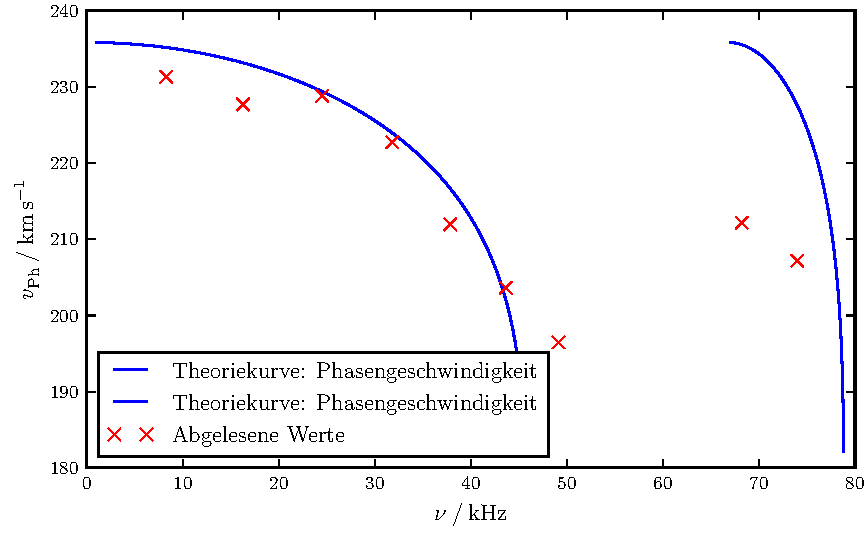
\includegraphics{eigenfrequenzen.pdf}
  \caption{Phasengeschwindigkeiten der Eigenfrequenzen der LC-Kette sowie dazugehörige Theoriewerte.}
  \label{fig:phasengeschwindigkeiten}
\end{figure}
Für die Theoriekurve ergeben sich zwei Abschnitte des Graphen, da die Phasengeschwindigkeit im Bereich der Grenzfrequenzen nicht definiert ist.
Es fällt direkt auf, dass es, abgesehen vom dritten Messwert, starke systematische Abweichungen der Phasengeschwindigkeiten nach unten gibt.
Dieser Sachverhalt, und die Tatsache, dass es sich nicht um einen Fehler in der theoretischen Betrachtung handelt, werden in der Diskussion genauer beleuchtet.

\subsection{Bestimmung der Form der stehenden Wellen}
Um die Form der stehenden Wellen zu analyiseren, werden, wie in der Durchführung beschrieben, die Amplituden der einzelnen Kondensatoren betrachtet.
Exemplarisch wird die Form der stehenden Wellen für die Frequenzen
\begin{align*}
  \nu_1 &= \SI{7806}{\hertz} & \nu_2 &= \SI{15540}{\hertz}
\end{align*}
betrachtet.
Hierzu werden die gemessenen Spannungen an den Kapazitäten gegen die jeweilige Nummer $n$ des Kondensators abgetragen, wobei zu beachten ist, dass die Spannungen jeweils den Effektivwert der Spannung darstellen.
In Tabelle \ref{tab:stehend1} sind die gemessenen Werte angegeben.
\begin{table}
  \centering
  \caption{Gemessene Spannungen an den einzelnen Kondensatoren der $LC$-Kette für die Eigenfrequenzen $\nu_1$ und $\nu_2$.}
  \label{tab:stehend1}
  \sisetup{table-format=1.2}
  \begin{tabular}{c c c}
    \toprule
    {$n$} & {$U_{\nu_1} [\si{\volt}]$} & {$U_{\nu_2} [\si{\volt}]$}\\
    \midrule
    \input{build/dtabelle.tex}
    \bottomrule
  \end{tabular}
\end{table}

Zudem wird die erwartete stehende Welle, welche sich nach Formel \ref{eqn:ste_1} berechnet, eingetragen.
Die Daten sind in den Abbildungen \ref{fig:stehend1} sowie \ref{fig:stehend2} dargestellt.

\begin{figure}[H]
  \centering
  \includegraphics{stehende_welle_1.pdf}
  \caption{Form der stehenden Welle für die Eigenfrequenz $\nu_1$.}
  \label{fig:stehend1}
\end{figure}

\begin{figure}[H]
  \centering
  \includegraphics{stehende_welle_2.pdf}
  \caption{Form der stehenden Welle für die Eigenfrequenz $\nu_2$.}
  \label{fig:stehend2}
\end{figure}

Wird das Experiment, wie in der Durchführung beschrieben, mit zugeschalteten Wellenwiderstand für $\nu_1$ durchgeführt, ergeben sich erwartungsgemäßg stehende Wellen der in Formel \ref{eqn:ste_2} angegebenen Form, das heißt mit Spannungsknoten am Ende und Anfang der $LC$-Kette.
Die gemessenen Werte sind in Tabelle \ref{tab:stehend2} angegeben.
\begin{table}[H]
  \centering
  \caption{Gemessene Spannungen an den einzelnen Kondensatoren der $LC$-Kette für die Eigenfrequenz $\nu_1$ bei zugeschalteten Wellenwiderstand.}
  \label{tab:stehend2}
  \sisetup{table-format=1.2}
  \begin{tabular}{c c}
    \toprule
    {$n$} & {$U_{\nu_1} [\si{\milli\volt}]$}\\
    \midrule
    \input{build/dtabelle2.tex}
    \bottomrule
  \end{tabular}
\end{table}
Da sich ein nicht unerheblicher Offset bei der Spannung ergibt, werden in Abbildung \ref{fig:stehend3} die gemessenen Werte ohne Theoriekurve angegeben.

\begin{figure}[H]
  \centering
  \includegraphics{stehende_welle_3.pdf}
  \caption{Form der stehenden Welle für die Eigenfrequenz $\nu_1$ mit zugeschaltetem Wellenwiderstand.}
  \label{fig:stehend3}
\end{figure}
